\graphicspath{ {./figuresMeasure} }
\section{Measure}

\subsection{Conception}
Afin de valider nos simulation nous allons procédé aux mesures de quelque configuration choisi. 6 PCB seront fabriqué. Nous avons choisi de représenter un nombre de piste de 10 et 5. Car nos simulation de 20 piste nous donne une capacité beaucoup trop élever. Pour chaque nombre de piste nous prenons deux rapport largeur et distance déjà simulé plus un plus faible pour étudié la possibilité de détecté de petite goutte. Le plan de cuivre du dessous est gardé pour tous. Pour les mesures les carte seront posé à plat nous ne voulons pas que ce qui se trouve en dessous aie une influence. Chaque PCB se verra attribué une lettre pour faciliter, par la suite, le nommage.

\begin{table}[!ht]
\begin{center}
\begin{tabular}[c]{lllll}
PCB & Nb piste & rapport larg/dist & Largeur de piste [mm] & distance entre piste [mm] \\
\hline
A & 10 & 2 & 4 & 2\\
B & 10 & 0.5 & 2 & 4\\
C & 10 & 0.22 & 1.1 & 4.9\\
D & 5 & 1 & 6 & 6\\
E & 5 & 0.5 & 4 & 8\\
F & 5 & 0.1 & 1.1 & 10.9
\end{tabular}
\caption{Liste des configurations sélectionné }
\end{center}
\end{table}

Le pcb est construit en suivant le plan mécanique de la figure \ref{plan}. Nous avons ajouté deux connecteurs SMB pour le relié à la carte de développement du convertisseur. Ils ont ensuite été pannelisé afin de les produire en une commande.

\begin{figure}[!ht]
\centering
 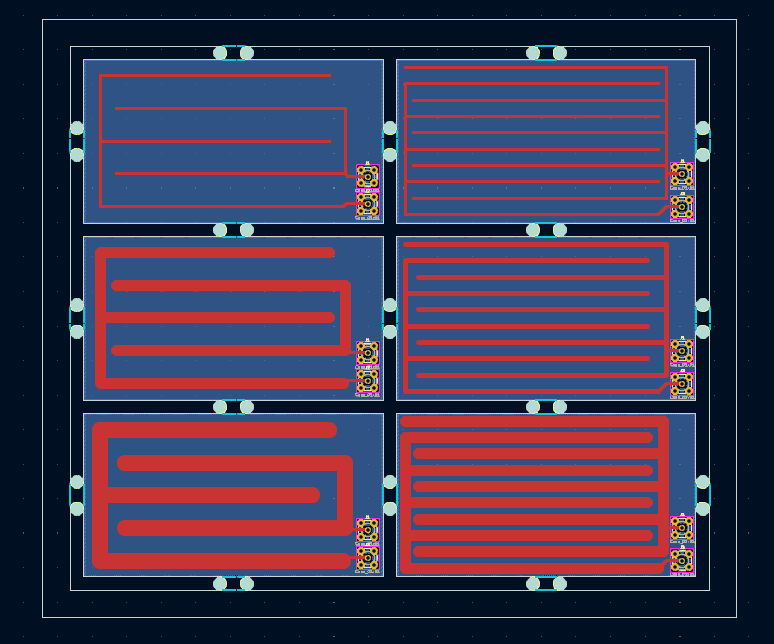
\includegraphics[width=10cm]{pannel.png}
 \caption{Pannel prêt à la production}
\end{figure}

\newpage

\subsection{Measure capacitive par filtre RC}

Avant de brancher nos cartes sur le convertisseur, nous allons effectuer une première mesures de la capacité afin de s'assure si nous somme ou non a l'intérieur des bornes. Nous n'avons pas a notre disposition un analyseur d’impédance capable de mesurer de si faible capacité. Nous placerons la capacité à mesuré dans un filtre RC et déterminerons son temps de charge. Nous utiliserons un microcontrôleur pour généré un signal carré. Il faudra prendre en compte l’impédance et la capacité de la sonde d'oscilloscope car nous somme dans le même ordre de grandeur.


\begin{figure}[!ht]
\centering
 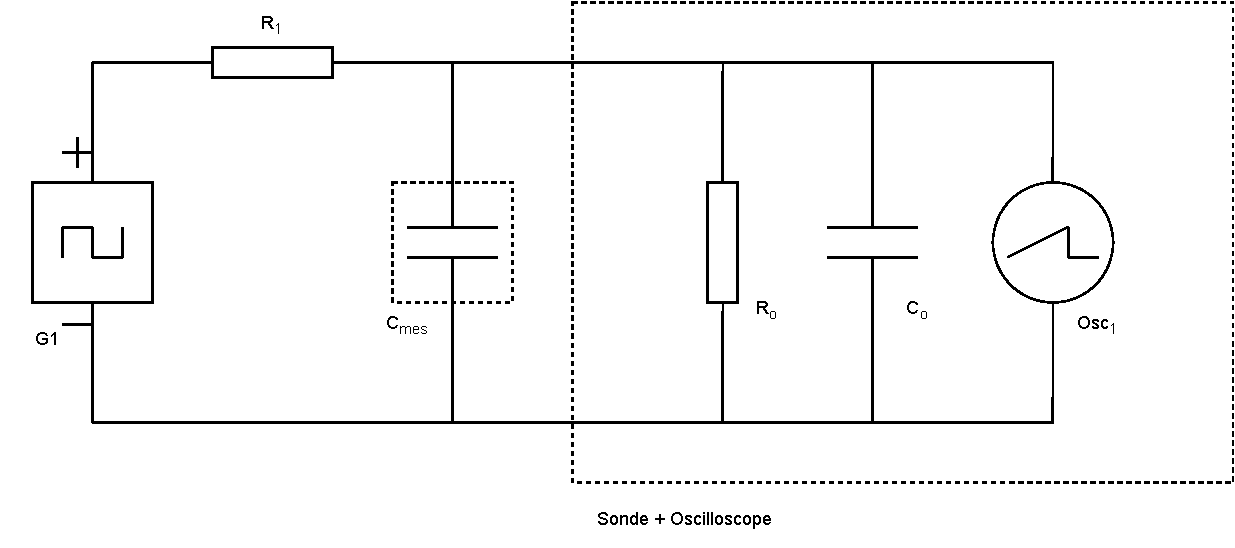
\includegraphics[width=10cm]{schemaMesure.pdf}
 \begin{description}
 \item[G1] uController STM32 signal 3.3V
 \item[R1] 1 M ohm
 \item[C$_{mes}$] PCB A,B,C,D,E,F
 \item[R$_o$] 10 M ohm
 \item[C$_o$] TBD
 \item[Osc$_1$] Picoscope 6043CD
\end{description}
 \caption{Schéma de mesure du filtre RC}
\end{figure}

L'impédance de la sonde et de l'oscilloscope est fourni mais la capacité est variable par la calibration de la sonde. Nous allons effectué une première mesure à vide sans $C_{mes}$ afin de déterminer $C_o$


\begin{figure}[!ht]
\centering
 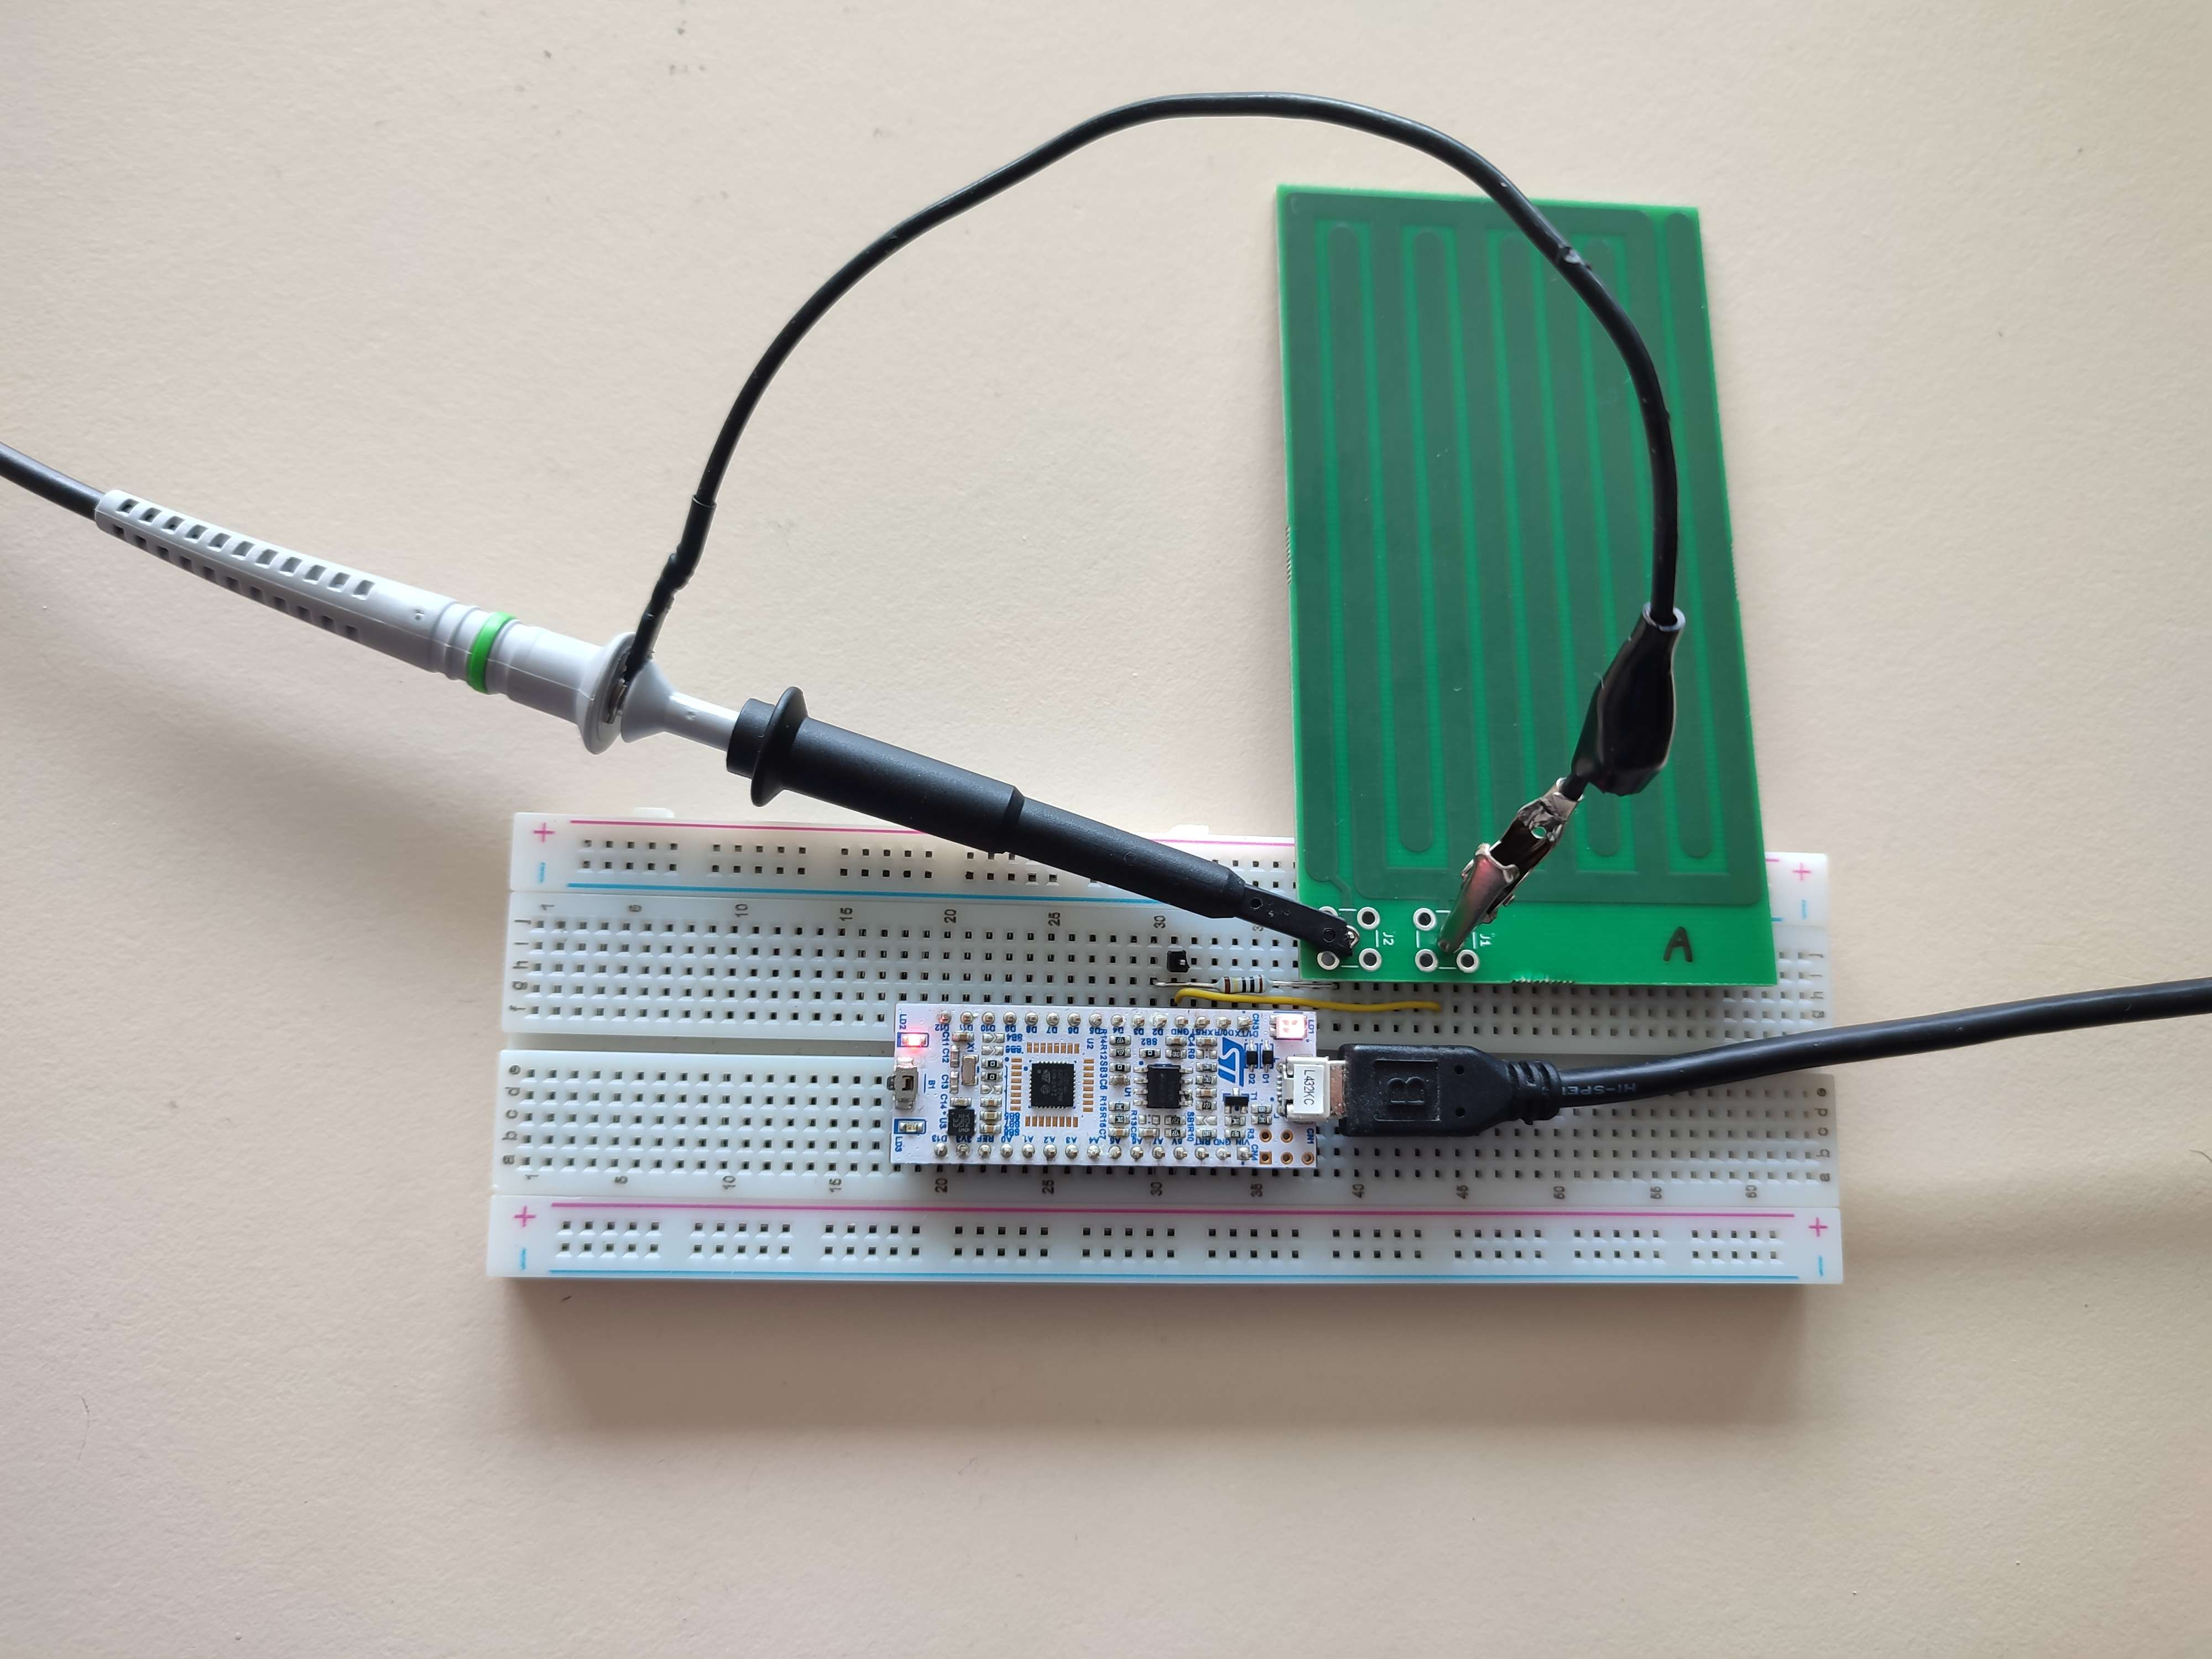
\includegraphics[width=10cm]{RCPhoto.jpg}
 \caption{Photo de la mesure RC}
\end{figure}

\newpage

Pour déterminer la constante de temps nous utilisons le résultat de la résolution de l'équation différentiel d'un circuit RC: 

\begin{equation}
 U_{c}(t) = U_{in} \cdot (1 - e^{-\frac{t}{RC}})
\end{equation}
On pose $t = RC$
\begin{equation}
\frac{U_c(RC)}{U_{in}} = 1 - e^{-1} = 1 - 0.37 = 0.63
\end{equation}

 $U_c$ vaudra 63\% de $U_{in}$ 

 
Si on prend en compte la sonde et l'oscilloscope le circuit de mesure n'est pas un simple RC. Nous le simplifions par un schéma équivalent grâce à Thévenin. 
 
\begin{equation}
 R_{th} = R_1 // R_o = \frac{1}{\frac{1}{R_1} + \frac{1}{R_o}} = 909 [k\Omega]
\end{equation}

\begin{equation}
 U_{th} = U_{G1} * \frac{R_o}{R_1 + R_o} = 3 [V]
\end{equation}

Le schéma équivalent que nous utiliserons pour les calculs est le suivant:

\begin{figure}[!ht]
\centering
 \includegraphics[width=10cm]{schemaMesureTH.pdf}
 \begin{description}
 \item[R$_{th}$] 909$[k\Omega]$
 \item[U$_{th}$] 3[V]
\end{description}
 \caption{Schéma équivalent Thévenin de mesure du filtre RC}
\end{figure}

$C_{mes}$ et $C_o$ se combine. En laissant vide $C_{mes}$ nous pouvons déterminer $C_o$. Nous le soustrairons aux prochaine mesures pour déterminer $C_{mes}$.

\begin{figure}[!ht]
\centering
 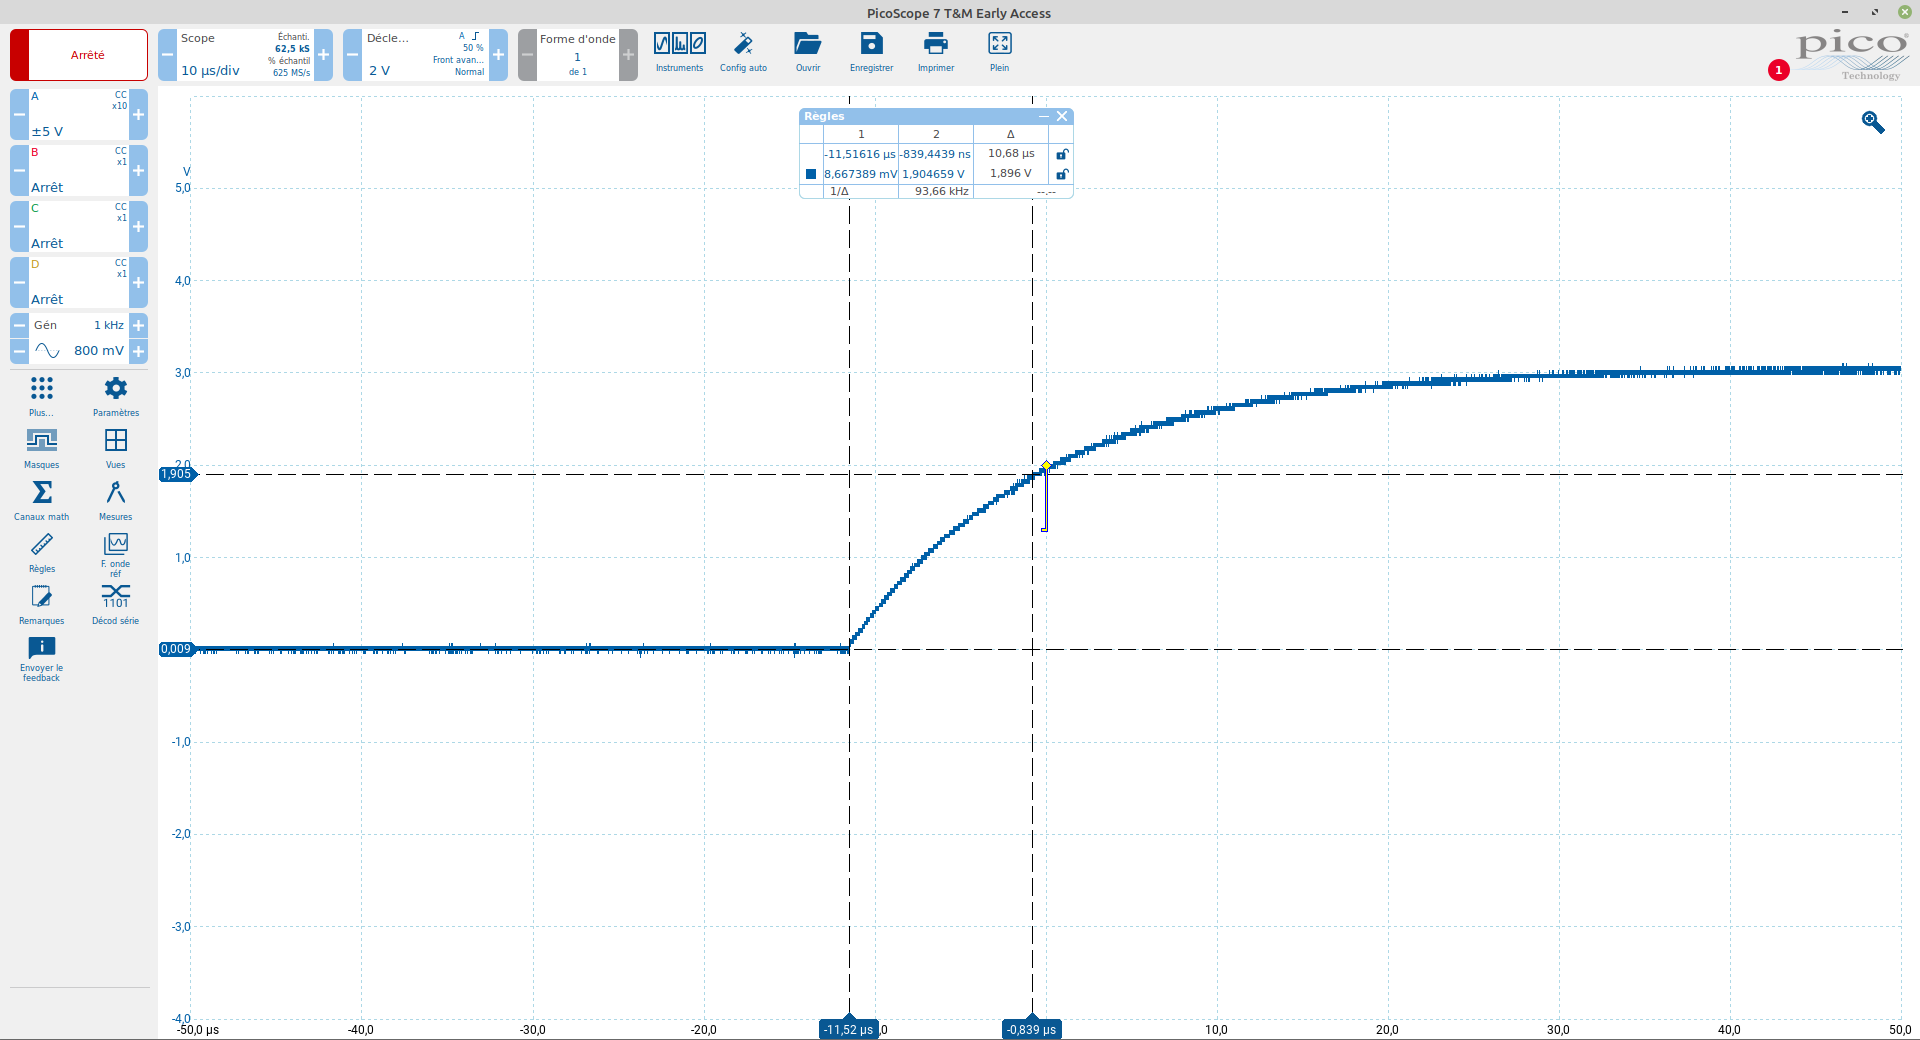
\includegraphics[width=14cm]{videe.png}
 \caption{Oscillogramme sans plaque}
\end{figure}

A 63\% de $U_{th}$ c'est à dire à 1.89 V nous observons un temps de \SI{10.68}{\micro\second} ce qui correspond à une capacité de $C_o = \frac{\tau}{R_{th}}= \SI{11.75}{\pico\farad}$. Nous pouvons à présent mesuré tous nos carte la même technique de mesure et en utilisant l'expression suivante:

\begin{equation}
 C_{mes} = \frac{\tau}{R_{th}} - C_o
\end{equation}

Nous pouvons aussi comparer, lorsque cela est possible, ces mesures à nos simulations. 

\begin{table}[!ht]
\begin{center}
\begin{tabular}[c]{lll}
PCB & Mesure RC [pF] & Simulation [pF]\\
A & 47.3 & ×\\
B & 29.9 & ×\\
C & 23.2 & ×\\
D & 29.9 & 26.4\\
E & 23.2 & 19.9\\
F & 11.9 & ×
\end{tabular}
\caption{Résumé des mesures et de la simulation pour chaque carte }
\end{center}
\end{table}


Les mesures sont proche de la simulation, on note une différence de 10\% à 20\%. Cette variation peut s'expliquer par plusieurs choses. D'une part la simulation prenais en compte une coupe mais sur nos carte des pistes supplémentaires sont présente aux extrémité pour connecter les lignes. Le connecteur peut aussi ajouter une capacité non négligeable. De plus notre mesure n'est pas parfaite et nous avons simplifié l'effet que peut avoir la sonde et l'oscilloscope. Nous somme dans un ordre de grandeur avec de très faible courant. La mesure est facilement influençable par des grandeur parasite que nous négligeons habituellement. 

Ces mesures nous donne une certaine confiance dans nos simulation. Nous pourrons en refaire de plus complexe dans une suite du projet tout en ayant une idée de comment les résultat se traduise dans la réalité.  


\subsection{Convertisseur Capacitif}

Nous pouvons à présent essayer le convertisseur AD7150. Nous utiliserons sa carte de développement EVAL-AD7150. La carte est fourni avec un logiciel pour configurer et effectuer directement des mesures. Nous pouvons nous passer de microcontrôleur pour l'instant. s

Nous allons commencer par mesurer la carte F. C'est la seul qui rentre dans les borne du convertisseur et pourra être mesuré directement. 

\begin{figure}[!ht]
\centering
 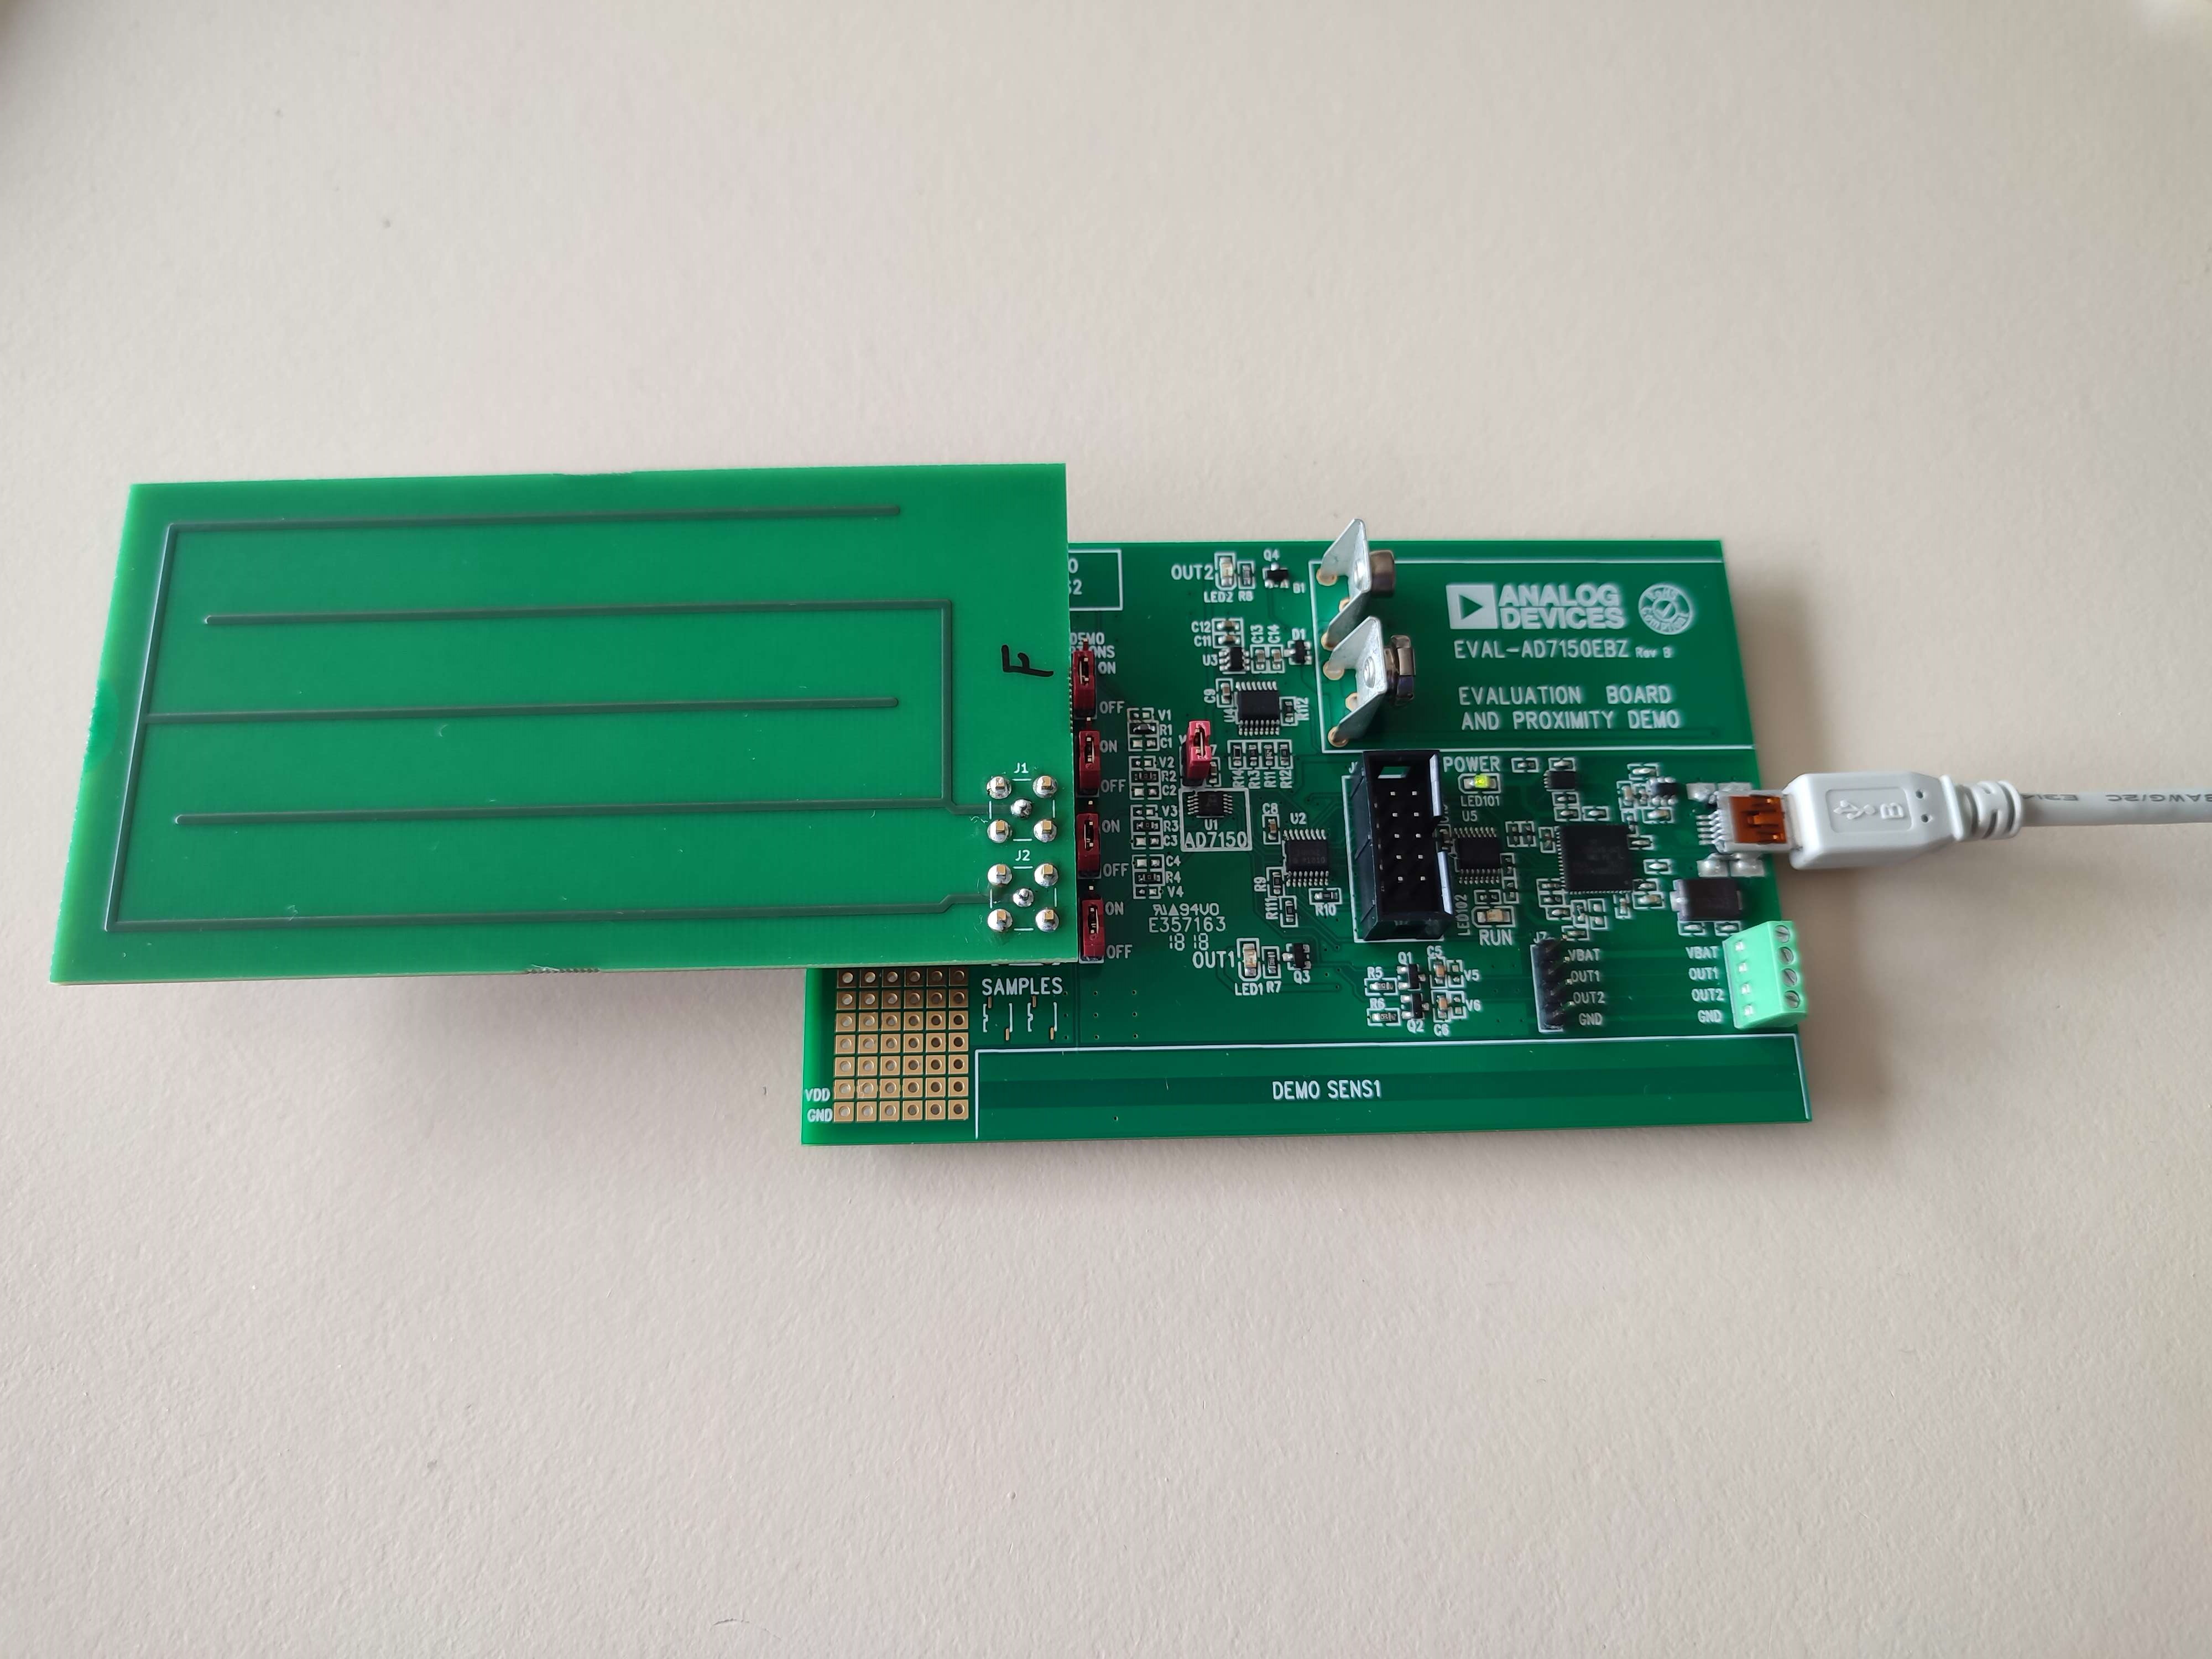
\includegraphics[width=10cm]{ADPhoto.jpg}
 \caption{Photo de la mesure de F avec EVAL-AD7150}
\end{figure}

\newpage

Pour cette première mesure le convertisseur est configuré avec une sensibilité de 2pF. Le CapDAC qui est l'offset est trouvé en le modifiant jusqu'à que la mesure ne sature plus. 

\begin{figure}[!ht]
\centering
 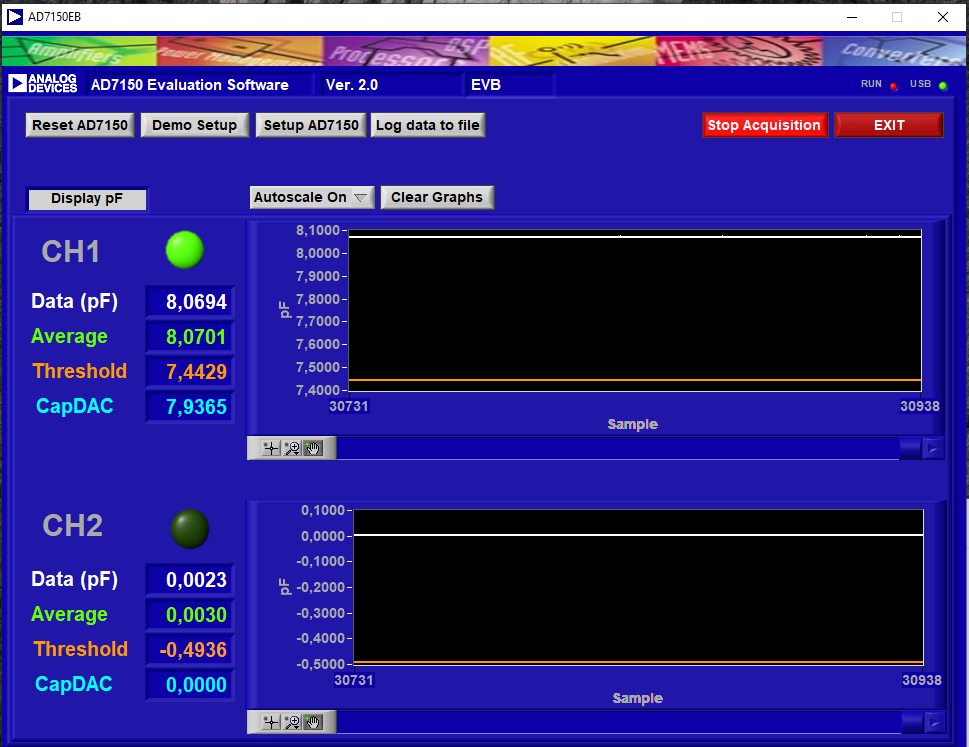
\includegraphics[width=10cm]{Fadair.png}
 \caption{Mesure de la carte F avec l'interface de la carte de développement de l'AD7150  }
\end{figure}

Nous mesurons une capacité de 8.1 pF pour 11.9 pF mesuré par RC. Cette différence s'explique d'une part par la précision d'une mesure RC expliqué précédemment et d'une autre par problème propre au convertisseur AD7150. 

Nous avons remarqué lors de nos mesure que lorsque nous approchons la main de la carte la capacité mesuré diminue fortement ce qui ne se produisait pas avec le filtre RC. Cela viens de l’influence de la capacité parasite à la masse. Aucun des deux pôle de la carte ne sont relié à la masse. Si une capacité apparaît entre un des pôle et la masse des charge seront perdue et ne seront pas mesuré par le convertisseur ce qui diminuera la capacité observé. Même si nous somme éloigner du capteur une capacité parasite est présente en partie à cause du plan de masse de la carte de développement. Nous ne pourrons malheureusement pas mesurer correctement la capacité absolue de nos cartes. 

Nous pouvons cependant commencer à détecter à titre indicatif des gouttes d'eau. 

\begin{figure}[!ht]
\centering
 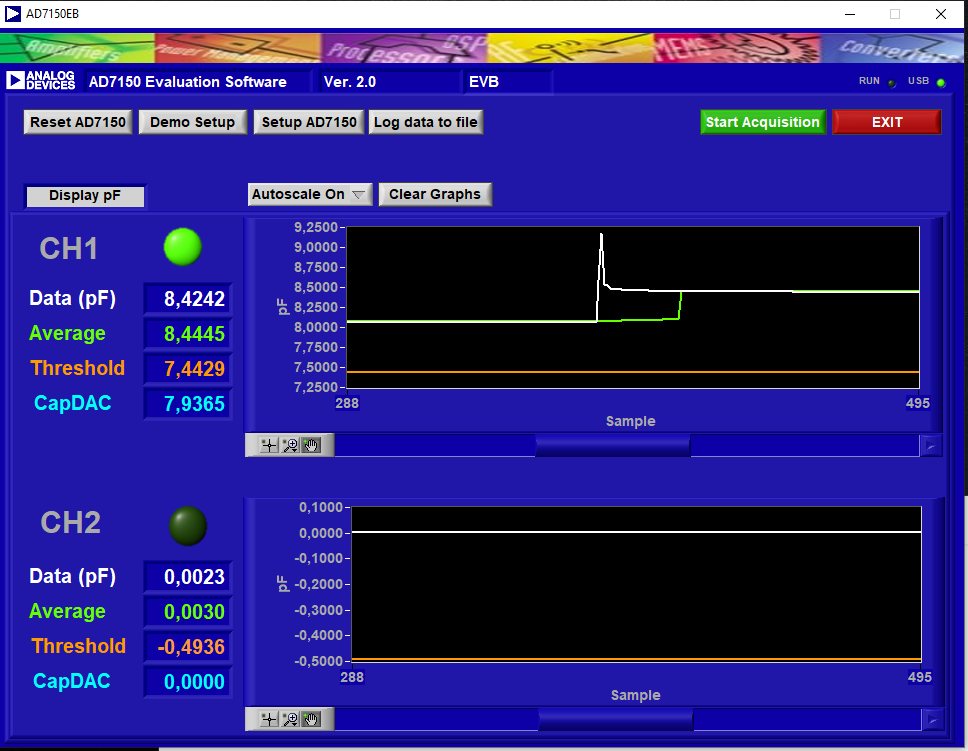
\includegraphics[width=10cm]{fadeau.png}
 \caption{Mesure de la carte F en faisant tomber une goutte d'eau}
\end{figure}

\newpage
Ces mesures ne permettent pas de sortir des chiffre précis mais nous introduis le comportement de l'eau sur notre capteur. Pour pouvoir essayer les autre carte malgré qu'elles soient hors borne nous avons mis une capacité de 10pF en série avec notre dipôle. Sur la carte de développement nous remplaçons par notre capacité une résistance de 0 ohm qui fait le pont entre le convertisseur et le connecteur. La capacité parasite de masse est trop compliqué à calculé dans cette configuration. Nous prendrons pas en compte la valeur absolue de la mesure mais seulement l’influence de l'eau. Il apparaît clairement qu'avec des pistes plus serré les gouttes son plus facilement détecter malgré la perte de sensibilité du à l'ajout d'une capacité en série. 
La taille et la position de la goutte influence beaucoup la détection de celle-ci. Un travail supplémentaire devra être effectué pour optimiser le peigne. La simulation en 2 dimension ne suffira pas pour représenté la géométrie et le placement d'une goutte d'eau.

